\documentclass{beamer}

\usepackage[serbian]{babel}

\usepackage{utopia} %font utopia imported
\usetheme{CambridgeUS}  
\usecolortheme{orchid}

\usepackage{amssymb,amsmath,amsthm}
\usepackage{tikz}

\newtheorem{teorema}{{Teorema}}[section]
\newtheorem{lema}{{Lema}}[section]
\theoremstyle{definition}
\newtheorem{primer}{{Primer}}
\newtheorem{definicija}{{Definicija}}

\renewcommand\qedsymbol{$\square$}

\setbeamercolor{block title}{use=structure,fg=white,bg=red!60!black}
\setbeamercolor{block body}{use=structure,fg=black,bg=red!5!white}
\setbeamercolor{section number projected}{fg=white,bg=red!60!black}
\setbeamertemplate{itemize item}{\color{red}$\bullet$}



\title{\bf Zna\v{c}ajne ta\v{c}ke trougla}
\author{Marija Kosti\'{c}}
\date{Matematik\v{c}ki fakultet, V smer}
\logo{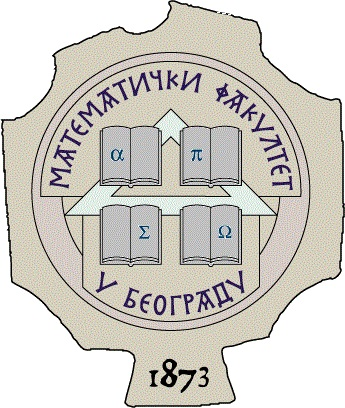
\includegraphics[height=1.5cm]{grbMATF.jpg}}

\AtBeginSection[]
{
  \begin{frame}
    \frametitle{\bf Zna\v{c}ajne ta\v{c}ke trougla}
    \tableofcontents[currentsection]
  \end{frame}
}

\begin{document}

\frame{\titlepage}

\begin{frame}
\frametitle{\bf Zna\v{c}ajne ta\v{c}ke trougla}
\tableofcontents
\end{frame}

\section{Centar opisanog kruga}

\begin{frame}
\frametitle{\bf Centar opisanog kruga}
		\begin{columns}[t]
			\column{0.6\textwidth}
			\pause
			\begin{definicija}
			\alert{\bf Simetrala stranice} trougla je prava koja je normalna na stranicu trougla i sadr\v{z}i sredi\v{s}te te stranice.
			\end{definicija}
			
			\pause
			\begin{teorema}[O centru opisanog kruga]
			Simetrale stranica trougla $ABC$ seku se u jednoj ta\v{c}ki $O$.
			\end{teorema}
			
			\column{0.4\textwidth}
			\begin{center}
				\resizebox{2in}{!}{\input{opisani.tkz}}
			\end{center}
		\end{columns}
		
		\pause 
		\begin{definicija} Ta\v{c}ka $O$ iz prethodne teoreme naziva se \alert{\bf centar opisanog kruga} trougla $ABC$.\pause Krug $k=k(O,r)$, gde je $r = OA = OB = OC$, naziva se \alert{\bf opisani krug} trougla $ABC$.
		\end{definicija}
		
\end{frame}

\section{Centar upisanog kruga}
\begin{frame}
\frametitle{\bf Centar upisanog kruga}
\begin{columns}[t]
	\column{0.45\textwidth}
	\pause
		\column{0.55\textwidth}
		
			\begin{definicija}
\alert{\bf Simetrala (bisektrisa)} unutra\v{s}njeg ugla trougla je prava koja polovi taj ugao.
\end{definicija}
			
\end{columns}


\end{frame}
\begin{frame}
\frametitle{\bf Centar upisanog kruga}
\begin{columns}[t]
	\column{0.45\textwidth}
	\begin{center}
				\resizebox{2.3in}{!}{\input{upisani.tkz}}
			\end{center}
		\column{0.55\textwidth}
		
			\begin{definicija}
\alert{\bf Simetrala (bisektrisa)} unutra\v{s}njeg ugla trougla je prava koja polovi taj ugao.
\end{definicija}
			
			\begin{teorema}[O centru upisanog kruga]
Simetrale uglova trougla $ABC$ seku se u jednoj ta\v{c}ki $S$.
\end{teorema}

			
		\end{columns}
		
			
\pause

\begin{definicija}
Ta\v{c}ka $S$ iz prethodne teoreme jednako je udaljena od stranica trougla $ABC$, pa je \alert{\bf centar upisanog kruga} u trougao $ABC$.
\end{definicija}   
\end{frame}

\section{Te\v{z}i\v{s}te}
\begin{frame}
\frametitle{\bf Te\v{z}i\v{s}te}
\pause
\begin{definicija}
\alert{\bf Te\v{z}i\v{s}na du\v{z} (medijana)} je du\v{z} koja spaja jedno teme trougla sa sredi\v{s}tem naspramne stranice.
\pause
Svaki trougao ima tri te\v{z}i\v{s}ne du\v{z}i.
\end{definicija}
\pause 
		\begin{center}
			\resizebox{1.8in}{!}{\input{teziste.tkz}}
		\end{center}
		
\end{frame}

\begin{frame} % teziste2

		\begin{teorema}[O te\v{z}i\v{s}tu]
Te\v{z}i\v{s}ne du\v{z}i trougla seku se u jednoj ta\v{c}ki $T$ koja ih delu u odnosu $2:1$.
\end{teorema}

		\begin{center}
			\only<2>{\resizebox{1.8in}{!}{\input{teziste1.tkz}}}
			% prvu sliku pokazi samo na pocetku dokaza, slajd 2
			\only<3-5>{\resizebox{1.8in}{!}{\input{teziste2.tkz}}}
			% drugu sliku prikazuj za vreme dokaza
			\only<1,6->{\resizebox{1.8in}{!}{\input{teziste3.tkz}}}
			% treca sliku prikazi sa tvrdjenjem teoreme (slajd 1) i kada je dokazemo (slajd 6)
		\end{center}
		
		\pause
		
		\begin{proof}
			\begin{itemize}
				\item<2-> Neka se  $BB_1,$ $CC_1$ seku u $T$;
				\item<3-> Neka su $C_2$ i $B_2$ sredi\v{s}ta $CT$ i $BT$;
				\item<4-> Tada je $C_1B_2C_2B_1$ paralelogram.  Zato je $T$ sredi\v{s}te $B_1B_2$ i $C_1C_2$;
				\item<5-> Dakle $T$ deli $BB_1$ i  $CC_1$ u odnosu $2:1$;
				\item<6-> Sli\v{c}no $T$ deli i $AA_1$ u odnosu $2:1$, pa tvrdjenje va\v{z}i.
				\qedhere
			\end{itemize}
		\end{proof}
		
	\end{frame} 
	
\begin{frame}
\begin{definicija}
Ta\v{c}ka $T$ iz prethodne teoreme naziva se \alert{\bf te\v{z}i\v{s}te trougla}.
\end{definicija}
    
\end{frame}

\section{Ortocentar}
\begin{frame}
\frametitle{\bf Ortocentar}
\pause
\begin{definicija}
Du\v{z} koja spaja teme trougla sa ta\v{c}kom preseka dveju normalnih pravih od kojih jedna prolazi kroz teme, a druga sadr\v{z}i naspramnu stranicu trougla naziva se \alert{\bf visina trougla}.\pause Posmatrana ta\v{c}ka preseka normalnih pravih naziva se \alert{\bf podno\v{z}je visine}. \pause Svaki trougao ima tri visine.
\end{definicija}
\pause
	\begin{center}
			\resizebox{2.5in}{!}{\input{visina.tkz}}
		\end{center}
		\end{frame}
		
\begin{frame}
\begin{teorema}[O ortocentru]
Prave odre\dj{}ene visinama trougla $ABC$ seku se u jednoj ta\v{c}ki $H$.
\end{teorema}
\pause
\begin{center}
			\resizebox{2.5in}{!}{\input{ortocentar2.tkz}}
		\end{center}
	
\end{frame}

\begin{frame}
\begin{teorema}[O ortocentru]
Prave odre\dj{}ene visinama trougla $ABC$ seku se u jednoj ta\v{c}ki $H$.
\end{teorema}

\begin{center}
			\only<1,2>{\resizebox{2in}{!}{\input{ortocentar3.tkz}}}
			% prvu sliku pokazi samo na pocetku dokaza, slajd 2
			\only<3>{\resizebox{2in}{!}{\input{ortocentar4.tkz}}}

		\end{center}
				%\pause
		
		\begin{proof}
			\begin{itemize}
				\item<1-> Neka su $PQ, QR$ i $RP$ paralelne redom stranicama $AB,BC$ i $AC$;
				\item<2-> Prema stavu $USU$, $\bigtriangleup ABC\cong\bigtriangleup PCB\cong\bigtriangleup CQA \cong\bigtriangleup BAR$ pa je $PC=CQ, QA=AR, RB=BF$;
				\item<3-> Jo\v{s} je $h_a \perp QR,h_b \perp PR, h_c \perp PQ$ pa su prave odre\dj{}ene visinama $\bigtriangleup ABC$ istovremeno simetrale stranica $\bigtriangleup PQR$;

			\end{itemize}
		\end{proof}
		
\end{frame}

\begin{frame}
\begin{teorema}[O ortocentru]
Prave odre\dj{}ene visinama trougla $ABC$ seku se u jednoj ta\v{c}ki $H$.
\end{teorema}

\begin{center}
	\only<1>{\resizebox{2in}{!}{\input{ortocentar4.tkz}}}			\only<2>{\resizebox{2in}{!}{\input{ortocentar5.tkz}}}

		\end{center}
				%\pause
		
		\begin{proof}
			\begin{itemize}

				\item<1-> Dakle po teoremi o centru opisanog kruga oko trougla $h_a, h_b$ i $h_c$ se seku u jednoj ta\v{c}ki $H$;
				\item<2-> Ta\v{c}ka $H$ je istovremeno ortocentar $\bigtriangleup ABC$ i centar opisanog kruga oko $\bigtriangleup PQR$.
				\qedhere
			\end{itemize}
		\end{proof}
    
\end{frame}



\begin{frame}
\begin{definicija}
Ta\v{c}ka $H$ iz prethodne teoreme naziva se \alert{\bf ortocentar trougla}.
\end{definicija}
\end{frame}


\end{document}